\subsection{Matrice de Gain}

La matrice de gain, correspondant aux valeurs clés, prises dans le cas
idéal de chaque responsable, est générée à partir des choix d'une
programmation mono-critères. \\

% TODO mettre une référence vers le mono-critère au lieu de ça
Prenant les stratégies de production pour chaque responsable comme suit :

\begin{itemize}
    \item Xcomptable = [235.625; 98.3929; 101.3393; 22.6786; 0; 50.625]
    \item Xcommercial = [0; 206.03; 43.26; 14.7; 70.97; 163.61]
    \item Xatelier = [0; 252.5; 195; 0; 0; 101.2500]
    \item Xstocks = 1.0e-16 * [0.5614; 0.2369; 0.114; 0.0365; 0.0028; 0.2099]
    \item Xpersonnel = [0; 0; 135.6644; 0; 0; 0]
\end{itemize}

Et retenant les anciennes fonctions à optimiser, on trouve :

$$
G =
\left (
    \begin{array}{ccccc}
        6473.2 & 362.1 & 508.7 & 2563.7 & 9487.4 \\
        5893.8 &     0 & 498.6 & 2494.4 & 9600.0 \\
        6130.2 & 346.3 & 548.7 & 2585.0 & 7331.2 \\
        0 &     0 &     0 &      0 &      0 \\
        2161.6 & 135.7 & 135.7 &  814.0 &      0
    \end{array}
\right )
$$

Les colonnes de cette matrice correspondent aux point de vues associés à chaque
responsable, c'est à dire la valeur lui important, il peut s'agir d'euros ou
d'unités produites, selon le responsable concerné. Les lignes quand à elles
correspondent à des stratégies de production à suivre, prises pour chaque
responsable, dans le même ordre que les colonnes. \\

On remarque que les valeurs se trouvant sur la diagonale correspondent à des
maximums/minimums, en l'occurence des optimums. Ceci confirme la validité de
la matrice de gain, car chaque responsable se trouve dans "son" cas optimal
à cet endroit.

\subsection{Équilibrage inter-critères}

En considérant le bénéfice comme variable "clé" intervenant dans ce problème,
l'optimisation des solutions se fait en procédant à une interpolation linéaire
entre le cas générant le plus de bénéfices, et le cas idéal pour chaque
responsable. \\

% TODO réparer le positionnement de l'image
%\begin{figure}
%    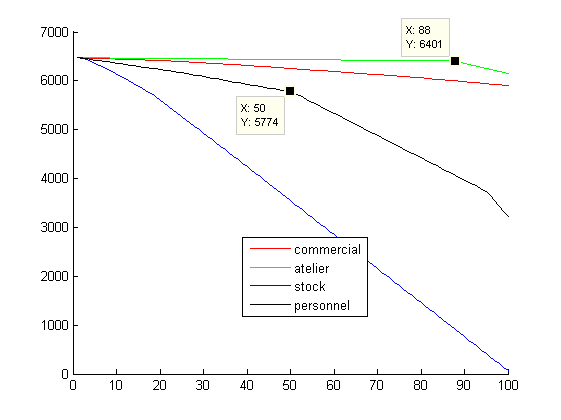
\includegraphics{graph_multi.png}
%    \caption{Graphe représentant l'évolution du bénéfice (en euros) par
%             rapport au pourcentage d'interpolation linéaire.}
%\end{figure}

Nous pouvons noter que les critères du responsable d'atelier et du responsable
commercial n'influent pas énormément sur le bénéfice, contrairement au
responsable des stocks, qui présente une corrélation linéaire avec la
diminution du bénéfice.
Nous remarquons que l'évolution du bénéfice en fonction du compromis pour les
responsables d'atelier et du personnel démarre par une décroissance faible
jusqu'à certaines valeurs de compromis "critiques" (respectivement 88\% et
50\%), ou la pente de dégression s'accroit. \\

De ce fait, nous ajusterons le compromis de ces derniers à ces valeurs limites,
afin qu'ils soient satisfaits au maximum, sans engendrer une perte trop
importante de bénéfice. \\

% TODO
